\documentclass[12pt,a4paper]{report}
\usepackage[utf8]{inputenc}
\usepackage[T1]{fontenc}
\usepackage{lmodern}
\usepackage{hyperref}
\hypersetup{
    colorlinks=true,
    linkcolor=blue,
    urlcolor=blue,
    citecolor=blue,
    pdfborder={0 0 0} % Removes the default red box around links
}
\usepackage{geometry}
\usepackage{fancyhdr}
\usepackage{enumitem}
\usepackage{amsmath, amssymb}
\usepackage{xcolor}
\usepackage{booktabs}
\usepackage{tikz}
\usetikzlibrary{positioning, shapes, arrows, calc, decorations.pathreplacing}
\usepackage{longtable}
\usepackage{array}
\usepackage{graphicx}
\usepackage{caption}
\usepackage{framed} % For framed boxes

% Custom colors
\definecolor{isygoblue}{RGB}{33, 150, 243}

% Page geometry
\geometry{
 a4paper,
 left=30mm,
 right=20mm,
 top=30mm,
 bottom=25mm,
}

% Header and footer
\pagestyle{fancy}
\fancyhf{}
\fancyhead[L]{\color{isygoblue}\textbf{ISYGO Consulting Services}}
\fancyhead[R]{\color{black}\textit{Week 1 - Day 1 Theory}}
\fancyfoot[C]{\color{isygoblue}\textit{Inspire Success, Your Goals \& Opportunities}}
\fancyfoot[R]{\thepage}

% Title page customization
\makeatletter
\def\maketitle{%
  \newpage
  \null
  \vfil
  \begin{center}%
  {\color{isygoblue}\LARGE \textbf{\@title}\par}
  \vspace{1cm}
  {\color{black}\large Week 1 - Day 1: Theory Guide \par}
  \vspace{0.5cm}
  {\color{isygoblue}\large \textit{Inspire Success, Your Goals \& Opportunities} \par}
  \vskip 2em%
  {\large
   \lineskip .5em%
   \begin{tabular}[t]{c}%
    \@author
  \end{tabular}\par
  }%
  \vskip 1.5em%
  {\large \@date \par}
  \end{center}
  \par
  \vfil
  \null
  \clearpage
}
\makeatother

\title{\color{isygoblue}\Huge\textbf{Expert Architecture Training Program}}
\author{\color{black}{ISYGO Consulting Services}}
\date{\color{black}{September 19, 2025}}

\begin{document}

\maketitle
\thispagestyle{empty}

\clearpage
\tableofcontents
\thispagestyle{empty}
\clearpage

\chapter*{Introduction}
\addcontentsline{toc}{chapter}{Introduction}
\markboth{Introduction}{Introduction}

Welcome to the \textbf{Expert Architecture Training Program}. This guide is designed to provide a \textbf{comprehensive understanding of Event-Driven Design (EDD)}, a paradigm where software components communicate through events—significant changes or occurrences in a system, such as "OrderPlaced" or "PaymentProcessed". Drawing from established sources like AWS and Confluent, EDD enables real-time information flow between microservices and devices, replacing polling with reactive, asynchronous notifications. Throughout this day, participants will delve into foundational concepts, advanced technologies, architectural patterns, best practices, and practical examples, building a robust foundation for designing, implementing, and managing event-driven architectures in enterprise-scale applications. As Solace notes, EDD decouples applications via event brokers, fostering agility in modern IT ecosystems.

\section*{Objectives of the Day}
\addcontentsline{toc}{section}{Objectives of the Day}
\markright{Objectives of the Day}

By the end of this training day, participants will be able to:  
\begin{enumerate}
    \item Define and explain Event-Driven Design (EDD) principles, including its core terminology like events, producers, and consumers, with references to real-world scalability gains.
    \item Identify the roles and interactions of producers, consumers, brokers, topics, partitions, and replicas within event-driven systems, exploring fault-tolerance mechanisms like ISR.
    \item Compare and contrast technologies such as Apache Kafka, RabbitMQ, and Pulsar, evaluating their trade-offs and use cases through benchmarks and architectural analyses.
    \item Apply best practices to ensure fault-tolerant, scalable, and maintainable event-driven systems, incorporating idempotency and schema evolution.
    \item Analyze multi-tenancy strategies, such as database-per-tenant or shared-schema approaches, and implement them effectively in hybrid environments.
    \item Monitor, test, and log event-driven applications using tools like Prometheus and the ELK stack, with strategies for tracing asynchronous flows.
    \item Connect theoretical concepts with real-world use cases, identifying common patterns and potential anti-patterns, from e-commerce inventory to banking fraud detection.
\end{enumerate}

\chapter{Event-Driven Design (EDD)}
\section{Definition and Overview}

Event-Driven Design (EDD), also known as Event-Driven Architecture (EDA), is an architectural approach where system components communicate asynchronously by producing and consuming \textbf{events}, defined as immutable records of significant state changes (e.g., "OrderPlaced", "PaymentProcessed", or "SensorTemperatureUpdated"). As per Confluent's introduction, EDA detects, processes, and reacts to real-time events, enabling loosely coupled systems that scale independently. This paradigm enhances \textbf{decoupling} by eliminating direct service calls, improves \textbf{scalability} through independent scaling of components, and boosts \textbf{responsiveness} by processing events without blocking, making it ideal for distributed, modern systems. AWS emphasizes that EDA encodes business actions into event notifications, supporting serverless and microservices patterns. Unlike request-response models, EDD promotes eventual consistency via patterns like event sourcing and CQRS, where reads and writes are segregated for performance.

\subsection{Real-World Example}
Consider an online e-commerce platform, as illustrated in GeeksforGeeks' system design:  
- The \textit{Order Service} generates an \texttt{OrderPlaced} event when a customer places an order, including details like item ID and quantity.  
- The \textit{Inventory Service} subscribes to this event to update stock levels in real-time, preventing overselling.  
- The \textit{Notification Service} uses the same event to send a confirmation email, while a \textit{Recommendation Engine} analyzes it for personalized suggestions.  
This asynchronous model ensures loose coupling, allowing each service to scale independently and handle failures gracefully. In practice, Netflix employs EDA for real-time recommendations, processing millions of viewing events daily to fan out suggestions across services, as noted in Solace's guide.

\section{Core Principles}
Drawing from AWS's best practices and Solace's complete guide, the core principles of EDD include:
\begin{enumerate}[label=\arabic*.]
    \item \textbf{Decoupling:} Producers and consumers operate independently, reducing dependencies and enabling separate evolution and scaling. Publishers send events once to a topic, with brokers distributing to subscribers, avoiding point-to-point integrations.
    \item \textbf{Asynchronous Communication:} Events are sent without waiting for immediate consumer action, preventing bottlenecks and enhancing throughput. This supports real-time reactions, as in Heineken's integration of 4,500 applications for logistics and payments.
    \item \textbf{Event Immutability:} Once published, events cannot be altered, ensuring consistency and enabling audit trails. As Medium's guide highlights, this facilitates replay for recovery without data corruption.
    \item \textbf{Durable Event Storage:} Events are persisted in brokers or logs, supporting replay for recovery or analytics. Tyk.io stresses using durable queues to handle failures gracefully.
    \item \textbf{Event Processing Modes:} Systems can handle events in real-time (streaming) or batch modes, tailored to specific business requirements. Additionally, Birlasoft adds idempotent processing to safely handle duplicates, and standardized schemas for evolution.
    \item \textbf{Loose Coupling and Scalability:} As per DEV Community's 10 principles, use JSON for evolutive payloads and topic hierarchies for filtering, ensuring subscribers receive only relevant events.
\end{enumerate}

\begin{framed}
\textbf{Astuce (Trick):} To optimize event throughput, pre-calculate partition counts based on expected load (e.g., ⌈total events / max consumer capacity⌉) and adjust dynamically with monitoring tools like Prometheus.
\end{framed}

These principles, when applied, transform rigid systems into resilient ones—imagine, how might idempotency prevent double-charging in a payment flow?

\section{Key Terminologies}
\begin{description}[style=nextline]
    \item[Event:] A timestamped, immutable record of a state change, such as \texttt{InvoiceGenerated}, carrying data like event type, payload, and metadata (e.g., source, timestamp). Confluent defines it as a notification of occurrences for real-time reaction.
    \item[Producer:] An application or service that generates and publishes events to a broker, e.g., using Kafka Producer API. Producers should publish once to one topic, per Solace's rules.
    \item[Consumer:] A service that subscribes to and processes events, such as a Kafka Consumer API implementation. Consumers filter via subscriptions, not business logic.
    \item[Topic:] A logical category or channel for grouping related events, enabling organized parallel processing. Topics use hierarchies (e.g., "ecommerce.orders.placed") for scalability.
    \item[Partition:] A subset of a topic that ensures ordered event processing and supports scalability across multiple consumers. Partitions enable horizontal scaling, with ordering per partition.
    \item[Broker:] A server or middleware (e.g., Kafka Broker) that stores, routes, and delivers events to consumers. Brokers manage replication for durability.
    \item[ISR (In-Sync Replica):] A Kafka-specific mechanism where replicas caught up to the leader form a set eligible for leadership election. As Confluent explains, writes commit only when all ISRs acknowledge, balancing durability and availability.
    \item[Schema Registry:] A centralized system (e.g., Confluent Schema Registry) storing event schemas (Avro, JSON, Protobuf) for structural consistency and backward compatibility during evolution.
    \item[Pub/Sub Pattern:] A messaging model where producers publish events to topics, and multiple consumers subscribe to receive them. AWS notes this as core to fan-out in microservices.
\end{description}

\subsection{Example Scenario}
In a banking application, as per IBM's overview:  
- A payment gateway produces \texttt{PaymentCompleted} events with details like transaction ID, amount, and account.  
- The fraud detection service analyzes these events in real-time for anomalies, using machine learning models triggered by the event.  
- The ledger service updates account balances based on the same events, ensuring atomicity via eventual consistency.  
This decoupled architecture minimizes inter-service dependencies, enhancing system resilience. ING Bank, for instance, uses EDA for fraud detection and personalized services, processing events across branches and apps for real-time alerts, reducing losses significantly.

\chapter{Messaging and Streaming Technologies}
\section{Overview}
Event-driven systems depend on messaging platforms that ensure reliable event delivery, persistence, and ordering. Key technologies include:

\begin{itemize}
    \item \textbf{Apache Kafka:} A distributed streaming platform optimized for high throughput (millions of events/sec), low latency, and durable event storage via log-based architecture. Developed at LinkedIn, it's ideal for event sourcing and analytics.
    \item \textbf{RabbitMQ:} A mature broker supporting AMQP, offering complex routing (e.g., exchanges) and guaranteed delivery. It's lightweight for traditional queuing but scales via clustering.
    \item \textbf{Apache Pulsar:} A cloud-native system with multi-tenancy and geo-replication, using BookKeeper for segmented storage. Originating from Yahoo, it separates compute from storage for elastic scaling.
\end{itemize}

These platforms, as benchmarked by Confluent, vary in architecture: Kafka's log-centric vs. Pulsar's tiered storage vs. RabbitMQ's queue model.

\section{Comparative Analysis}
To clarify trade-offs, consider this refactored single-column table, scaled to fit A4:

\begin{center}
\resizebox{\textwidth}{!}{%
\begin{tabular}{l p{10cm}}
\toprule
\textbf{Feature} & \textbf{Details} \\
\midrule
\textbf{Throughput} & Kafka: High (1M+ msgs/sec); RabbitMQ: Medium (10K-100K msgs/sec); Pulsar: High (1M+ msgs/sec) \\
\textbf{Latency} & Kafka: Low (ms); RabbitMQ: Low-Medium (ms); Pulsar: Low (ms) \\
\textbf{Persistence} & Kafka: Log-based (durable); RabbitMQ: Optional (queues); Pulsar: Segmented (BookKeeper) \\
\textbf{Scaling} & Kafka: Horizontal (partitions); RabbitMQ: Clustered nodes; Pulsar: Elastic (separate storage) \\
\textbf{Multi-Tenancy} & Kafka: Limited (namespaces); RabbitMQ: Limited (vhosts); Pulsar: Native (namespaces) \\
\textbf{Protocols} & Kafka: Kafka API; RabbitMQ: AMQP, MQTT, STOMP; Pulsar: Pulsar, AMQP, MQTT \\
\textbf{Use Case} & Kafka: Streaming, analytics; RabbitMQ: Task queuing, RPC; Pulsar: Geo-replication, cloud-native \\
\bottomrule
\end{tabular}
}
\caption{Comparison of Kafka, RabbitMQ, and Pulsar}
\end{center}

\begin{framed}
\textbf{Astuce (Trick):} When configuring topics, set the replication factor to match your fault-tolerance needs (e.g., 3 for 2 failures) and monitor ISR health to avoid leader imbalances.
\end{framed}

\section{Technology Trade-Offs}
- \textbf{Kafka:} Excels in high-volume streaming and analytics (e.g., Netflix's data pipelines) but requires complex setup with ZooKeeper; best for log retention and replay, per Confluent benchmarks showing 2x Pulsar's throughput in some workloads.
- \textbf{RabbitMQ:} Ideal for enterprise messaging with routing flexibility (e.g., task distribution), less suited for large-scale streaming; lightweight but struggles beyond 100K msgs/sec, as noted in ProjectPro comparisons.
- \textbf{Pulsar:} Offers multi-tenancy and geo-replication (e.g., Yahoo's global feeds), with a steeper learning curve due to BookKeeper; faster at high throughput than RabbitMQ, per Confluent tests, but ecosystem lags Kafka's connectors.

How might these trade-offs influence your choice for a global e-commerce system?

\chapter{Event Flow and Architecture}
\section{Basic Flow Diagram}
\begin{center}
\resizebox{\textwidth}{!}{%
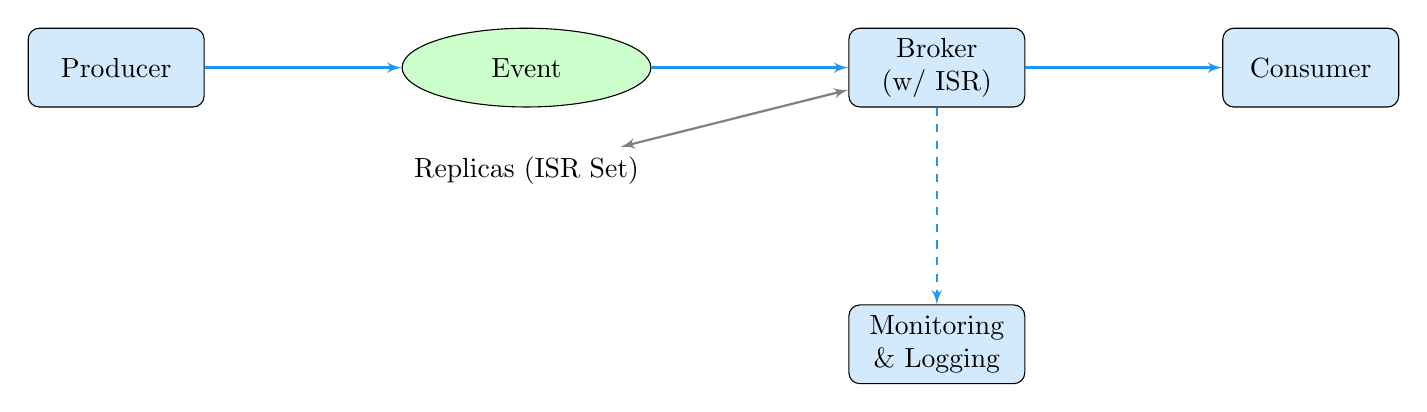
\begin{tikzpicture}[node distance=2.5cm, auto, >=latex']
    \tikzstyle{component} = [rectangle, draw, fill=isygoblue!20, rounded corners, minimum height=1cm, text width=2cm, align=center]
    \tikzstyle{event} = [ellipse, draw, fill=green!20, minimum height=1cm, text width=2cm, align=center]
    
    \node[component] (producer) {Producer};
    \node[event, right=of producer] (event) {Event};
    \node[component, right=of event] (broker) {Broker (w/ ISR)};
    \node[component, right=of broker] (consumer) {Consumer};

    \draw[->, thick, color=isygoblue] (producer) -- (event);
    \draw[->, thick, color=isygoblue] (event) -- (broker);
    \draw[->, thick, color=isygoblue] (broker) -- (consumer);
    
    \node[component, below=of broker] (monitor) {Monitoring \& Logging};
    \draw[->, thick, dashed, color=isygoblue] (broker) -- (monitor);
    
    \node[below=0.5cm of event] (replica) {Replicas (ISR Set)};
    \draw[<->, thick, color=gray] (broker) -- (replica);
\end{tikzpicture}
}
\end{center}
\caption{Event Flow in EDD with ISR Replication}
\clearpage

\begin{framed}
\textbf{Technical Note:} ISR ensures fault tolerance by maintaining synchronized replicas. Monitor ISR shrinkage (via \texttt{kafka-topics --describe}) to detect under-replicated partitions, indicating potential data loss risks.
\end{framed}

This diagram, resized to fit the page, illustrates the flow: Producers emit events to brokers, which replicate via ISR for fault tolerance, before consumers process them asynchronously.

\chapter{Multitenancy in Event-Driven Systems}
\section{Definition}
Multitenancy allows multiple tenants—distinct client groups or organizations—to share infrastructure while maintaining \textbf{logical isolation} of data and operations through separate namespaces or schemas. As Microsoft Learn describes, it balances cost-efficiency with isolation, using models like trusted (shared namespaces) vs. hostile (dedicated) for Event Hubs.

\section{Strategies}
\begin{itemize}
    \item \textbf{Database-per-tenant:} Each tenant has a dedicated database, offering maximum isolation but challenging scalability at high tenant volumes; suitable for sensitive data like banking.
    \item \textbf{Schema-per-tenant:} Uses one database with separate schemas per tenant, balancing isolation and manageability; Azure recommends for moderate workloads.
    \item \textbf{Shared-database, shared-schema:} All tenants share a single database and schema, requiring code-level isolation (e.g., tenant IDs in events); cost-effective but risky for noisy neighbors, per Frontegg's pros/cons.
    \item \textbf{Hybrid Approaches:} Combine strategies, e.g., shared brokers with tenant-specific topics in Pulsar, as in SAP BTP's CAP for event mesh.
\end{itemize}

Trade-offs include security (higher in isolated models) vs. cost (lower in shared), with auditing essential for compliance.

\section{Case Study: Tenant Document Processing}
A tenant uploads 1TB of PDFs daily. The upload service produces \texttt{DocumentUploaded} events to a Kafka topic with 10 partitions, calculated as \(\lceil 1 \, \text{TB} / (100 \, \text{MB/s} \times 3600 \, \text{s}) \rceil \approx 10\), assuming a consumer capacity of 100MB/s over a 1-hour processing window (3600 seconds). The OCR service consumes events in parallel, processing 100K PDFs/hour, with results stored in a data lake for analytics. This setup leverages Kafka's scalability, with partitions distributing load across consumers.\autocite{kafka2025}

\chapter{Monitoring, Logging, and Testing}
\section{Monitoring Metrics}
As Datadog's best practices outline, holistic EDA monitoring requires:
\begin{itemize}
    \item \textbf{Throughput:} Messages processed per second, tracked via DSM for end-to-end visibility.
    \item \textbf{Latency:} Time from event production to consumption, including broker delays.
    \item \textbf{Consumer Lag:} Unprocessed messages in partitions, alerting on backlogs.
    \item \textbf{Broker Health:} Disk usage, replication status, and ISR shrinkage.
    \item \textbf{Tools:} Prometheus/Grafana for metrics, Datadog DSM for stream tracing, CloudWatch for AWS integrations.
\end{itemize}

Centralize observability to trace asynchronous flows, correlating metrics with logs.

\section{Logging}
\begin{itemize}
    \item \textbf{Structured Logging:} Includes tenant ID, event context, and trace IDs for traceability in distributed systems.
    \item \textbf{Tools:} ELK stack for aggregation, Loki for lightweight querying, Splunk for advanced analytics.
    \item \textbf{Importance:} Essential for debugging asynchronous pipelines; TestRail stresses comprehensive logging to capture event paths in testing.
\end{itemize}

\section{Testing Strategies}
\begin{itemize}
    \item \textbf{Unit Tests:} Validate producer/consumer logic with JUnit/Mockito, simulating events.
    \item \textbf{Integration Tests:} Simulate brokers using Docker Compose/Testcontainers; DEV Community recommends event recording/replay for scenarios.
    \item \textbf{Schema Validation:} Ensure event compliance with registries before processing.
    \item \textbf{End-to-End Testing:} Use chaos engineering for fault injection, validating idempotency and ordering, per Tyk.io.
\end{itemize}

\chapter*{Evaluation Questions}
\begin{enumerate}
    \item How does event immutability, as in AWS EDA, enhance auditing in e-commerce inventory systems?
    \item Compare Kafka's ISR with Pulsar's BookKeeper for fault tolerance in banking fraud detection.
    \item What trade-offs arise in multi-tenant strategies for a global SaaS CRM, per Microsoft Learn?
    \item Design a monitoring setup using Datadog DSM to trace latency in a real-time payment flow.
    \item Why might RabbitMQ's routing excel over Kafka in task queuing, but falter in streaming analytics?
\end{enumerate}

\chapter*{Glossary}
\begin{itemize}
    \item \textbf{EDD/EDA:} Event-Driven Design/Architecture, using events for asynchronous communication.
    \item \textbf{ISR:} In-Sync Replicas, Kafka's set of synchronized replicas for durability.
    \item \textbf{AMQP:} Advanced Message Queuing Protocol, RabbitMQ's core standard.
    \item \textbf{Pub/Sub:} Publish/Subscribe pattern for event distribution.
    \item \textbf{Multitenancy:} Sharing infrastructure with isolated tenant data.
    \item \textbf{Kafka:} Distributed streaming platform for high-throughput events.
    \item \textbf{RabbitMQ:} Enterprise broker for queuing and routing.
    \item \textbf{Pulsar:} Cloud-native platform with geo-replication.
\end{itemize}

\chapter*{References}
\begin{itemize}
    \item \href{https://kafka.apache.org/documentation/}{Apache Kafka Documentation}\autocite{kafka2025}
    \item \href{https://www.rabbitmq.com/documentation.html}{RabbitMQ Documentation}
    \item \href{https://pulsar.apache.org/docs/}{Apache Pulsar Documentation}
    \item \href{https://martinfowler.com/articles/201701-event-driven.html}{Martin Fowler - Event-Driven Architecture}
    \item \href{https://solace.com/what-is-event-driven-architecture/}{Solace: The Complete Guide to Event-Driven Architecture}
    \item \href{https://aws.amazon.com/blogs/architecture/best-practices-for-implementing-event-driven-architectures-in-your-organization/}{AWS: Best Practices for EDA}
    \item \href{https://www.confluent.io/learn/event-driven-architecture/}{Confluent: EDA Introduction}
    \item \href{https://www.datadoghq.com/blog/monitor-event-driven-architectures/}{Datadog: Monitoring EDA}
    \item \href{https://www.geeksforgeeks.org/system-design/event-driven-architecture-system-design/}{GeeksforGeeks: EDA System Design}
    \item \href{https://tyk.io/learning-center/event-driven-architecture-best-practices/}{Tyk: EDA Best Practices}
    \item \href{https://dev.to/stack-labs/serverless-day-10-principles-for-your-event-driven-architecture-2lb7}{DEV Community: 10 EDA Principles}
    \item \href{https://www.birlasoft.com/articles/embracing-event-driven-architecture-core-principles-patterns-and-best-practices}{Birlasoft: EDA Principles and Best Practices}
    \item \href{https://www.confluent.io/blog/kafka-fastest-messaging-system/}{Confluent: Kafka vs. RabbitMQ vs. Pulsar Benchmark}
    \item \href{https://www.confluent.io/kafka-vs-pulsar/}{Confluent: Kafka vs. Pulsar Comparison}
    \item \href{https://streamnative.io/pulsar/what-is-pulsar}{StreamNative: Pulsar vs. Kafka}
    \item \href{https://learn.microsoft.com/en-us/azure/architecture/guide/multitenant/service/event-hubs}{Microsoft Learn: Multitenancy in Event Hubs}
    \item \href{https://www.testrail.com/blog/event-driven-application-architectures/}{TestRail: Testing EDA}
    \item \href{https://risingwave.com/blog/real-world-applications-of-event-driven-architecture-10-examples/}{RisingWave: Real-World EDA Examples}
    \item \href{https://www.ibm.com/think/topics/event-driven-architecture}{IBM: What is EDA?}
\end{itemize}

\end{document}